\documentclass[]{article}
\usepackage[a4paper, total={6in, 8in}]{geometry}
\usepackage[english]{babel}	
\usepackage[utf8]{inputenc} % Umlaute
\usepackage{amssymb}
\usepackage{amsmath} 
\usepackage{fancyhdr}
\usepackage{fancyvrb} % Für regex Umgebung
\usepackage{multicol} % Mehrere Spalten
\usepackage{graphicx} % bilder
\usepackage[table]{xcolor}
\usepackage{hyperref}
\pagestyle{fancy}
\fancyhf{} %clears the header and footer
\rhead{Professor Robert Feldmann (lectures) \\ Dr. Darren Reed (exercise classes) \\ Dimakopoulos Vasileios (TA) \\ Elia Cenci (TA)}
\lhead{Universität Zürich \\ Institute for Computational Science \\ Spring Semester 2021 \\ ESC403}
\fancyfoot[C]{\thepage}


\title{\textbf{INTRODUCTION TO DATA SCIENCE FINAL EXAM 2021}}
\author{Solutions from David Linder}

\begin{document}
	\maketitle
	\thispagestyle{fancy}
	\section{Time Series}
	\subsection{}
	To be considered stationary a time series should have the following properties:
	\begin{itemize}
		\item The mean $E[X_t]$ is the same for all times $t$
		\item The variance $Var[X_t]$ is the same for all times $t$
		\item The covariance between $X_t$ and $X_{t-1}$ is the same for all $t, n$
	\end{itemize}
	That means we want
	\begin{itemize}
		\item no obvious trends
		\item constant variance with time
		\item constant autocorrelation structure over time
		\item no periodic fluctuations (no seasonality)
	\end{itemize}
	I found some examples \href{https://otexts.com/fpp2/stationarity.html}{here}: In figure \ref{fig:time_series} we see that most of the series are non-stationary except series (b) and (g). In series (g) there are cycles but they are not periodic. 
	\begin{figure}
		\centering
		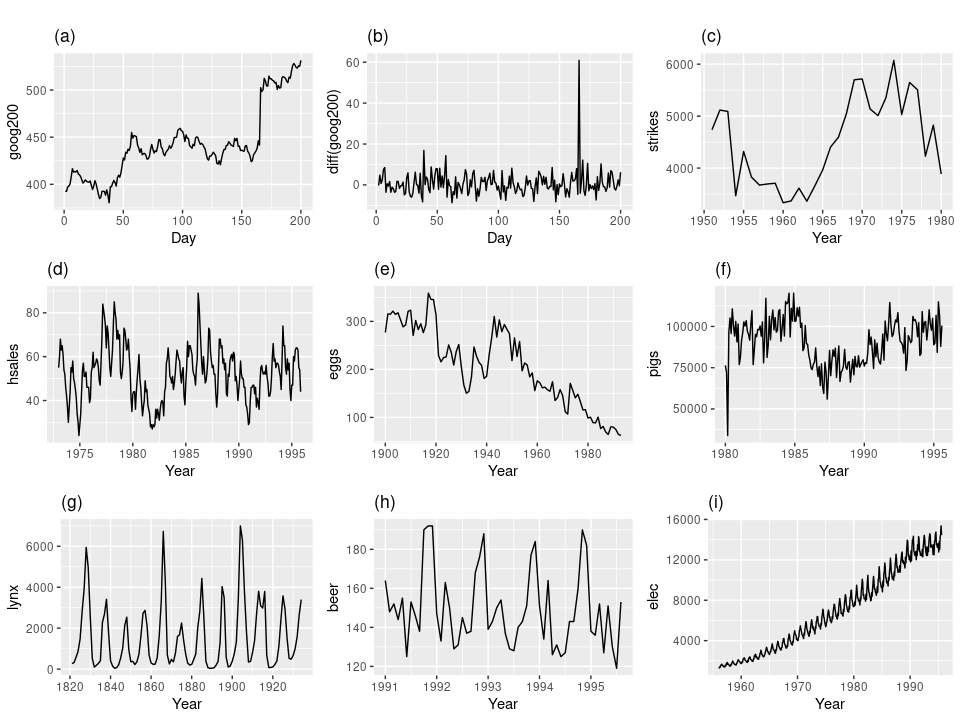
\includegraphics[width=0.8\textwidth]{images/time_series.png}
		\caption{(a) Google stock price for 200 consecutive days; (b) Daily change in the Google stock price for 200 consecutive days; (c) Annual number of strikes in the US; (d) Monthly sales of new one-family houses sold in the US; (e) Annual price of a dozen eggs in the US (constant dollars); (f) Monthly total of pigs slaughtered in Victoria, Australia; (g) Annual total of lynx trapped in the McKenzie River district of north-west Canada; (h) Monthly Australian beer production; (i) Monthly Australian electricity production.}
		\label{fig:time_series}
	\end{figure}
	
	\subsection{}
	
	\begin{itemize}
		\item By looking at the data we can clearly see that this time series is not stationary. After log transformed the $X$-data we can see in figure \ref*{fig:rollingmean} that although the standard deviation has a small variation the mean increases over time. Also the results of the Dickey-Fuller test is that we can not reject $H_0$ (TS is non-stationary) because the test statistic value is not less than the critical value. Here is the data in detail: 
		\begin{center}
			\begin{tabular}{|l|r|}
				\hline Test Statistic & $-0.2312$ \\
				\hline p-value & $0.9347$ \\
				\hline Lags & $22.0000$ \\
				\hline Observations & $975.0000$ \\
				\hline Critical Value $(1 \%)$ & $-3.4371$ \\
				\hline Critical Value $(5 \%)$ & $-2.8645$ \\
				\hline Critical Value $(10 \%)$ & $-2.5684$ \\
				\hline
			\end{tabular}
			\label{tab:dickey}
		\end{center}
		I will use the moving average smoothing method which we used in the exercise class to eliminate the trend. First i calculated the rolling mean with the pandas function and then subtracted this from the original series (code: timeseries/1.2.py). Then i dropped the nan values that resulted from averaging over the time window (i tried out different sizes of that window and ended up with a value of 60). In figure \ref{fig:rollingmean_diff} we see the result and that we eliminated the trend. Let's take a look at the test statistics:
		\begin{center}
			\begin{tabular}{|l|r|}
				\hline Test Statistic & $-10.7860$ \\
				\hline p-value & $0.0000$ \\
				\hline Lags & $1.0000$ \\
				\hline Observations & $937.0000$ \\
				\hline Critical Value $(1 \%)$ & $-3.4373$ \\
				\hline Critical Value $(5 \%)$ & $-2.8646$ \\
				\hline Critical Value $(10 \%)$ & $-2.5684$ \\
				\hline
			\end{tabular}
		\end{center}
		The value is lower than all the critical values. Therefore we can say at least with 99\% confidence this is now a stationary time-series.
		
		\begin{figure}
			\centering
			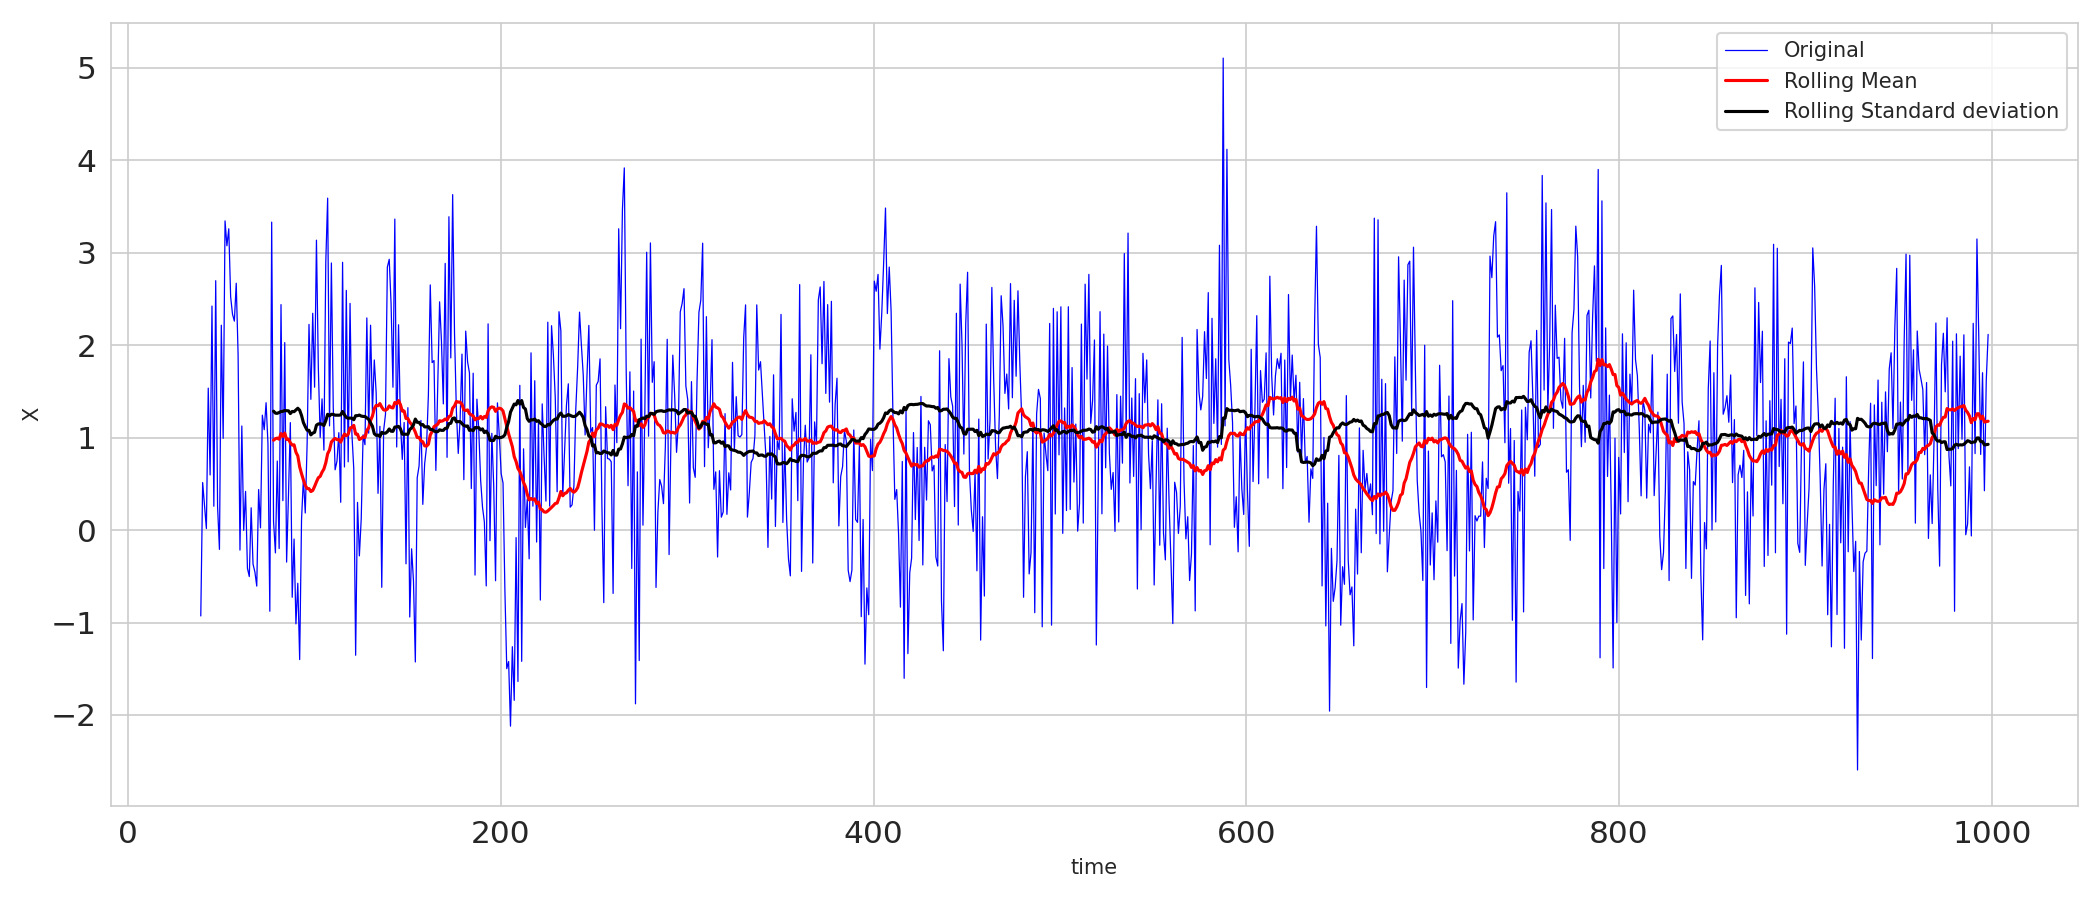
\includegraphics[width=1\textwidth]{images/ts_log_moving_avg_diff.png}
			\caption{The result from smoothing.}
			\label{fig:rollingmean_diff}
		\end{figure}
		\item For answering this question we need to find the p-value. For this value to find we look at the plot of the partial autocorrelation function (PACF). From figure \ref{fig:pacf} we find a p-value of 3. That means that 3 values of at prior times are expected to directly affet a given current value of the time series.
		\begin{figure}
			\centering
			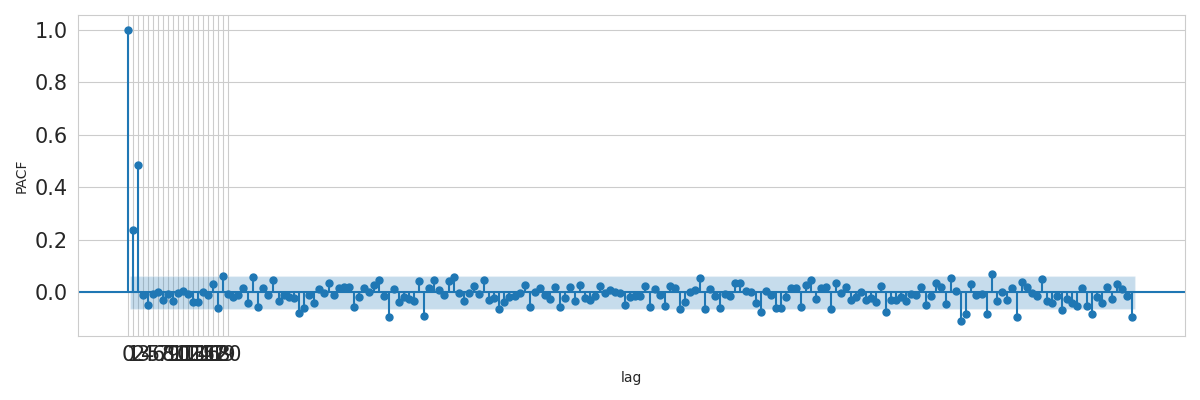
\includegraphics[width=1\textwidth]{images/partialautocorrelation.png}
			\caption{Plot of the partial autocorrelation function. The x-axis are the lags. One can see that the first time the PACF crosses the confidence interval (blue) is at lag 3.}
			\label{fig:pacf}
		\end{figure}
		\item 
		\begin{figure}
			\centering
			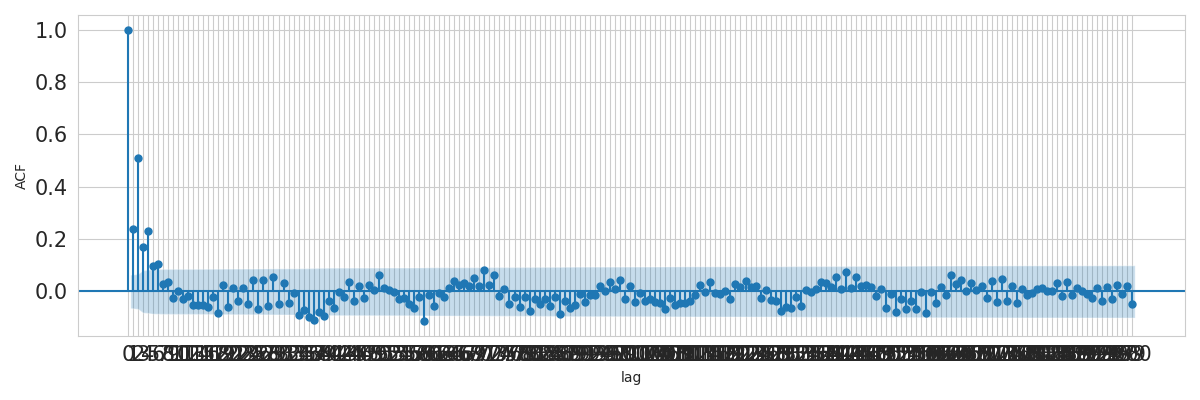
\includegraphics[width=1\textwidth]{images/autocorrelation.png}
			\caption{The autocorrelation function. The function crosses the confidence interval at lag 7 $\implies q=7$.}
			\label{fig:acf}
		\end{figure}
	\end{itemize}
	
	\subsection{}
	\begin{itemize}
		\item 
		\begin{figure}
			\centering
			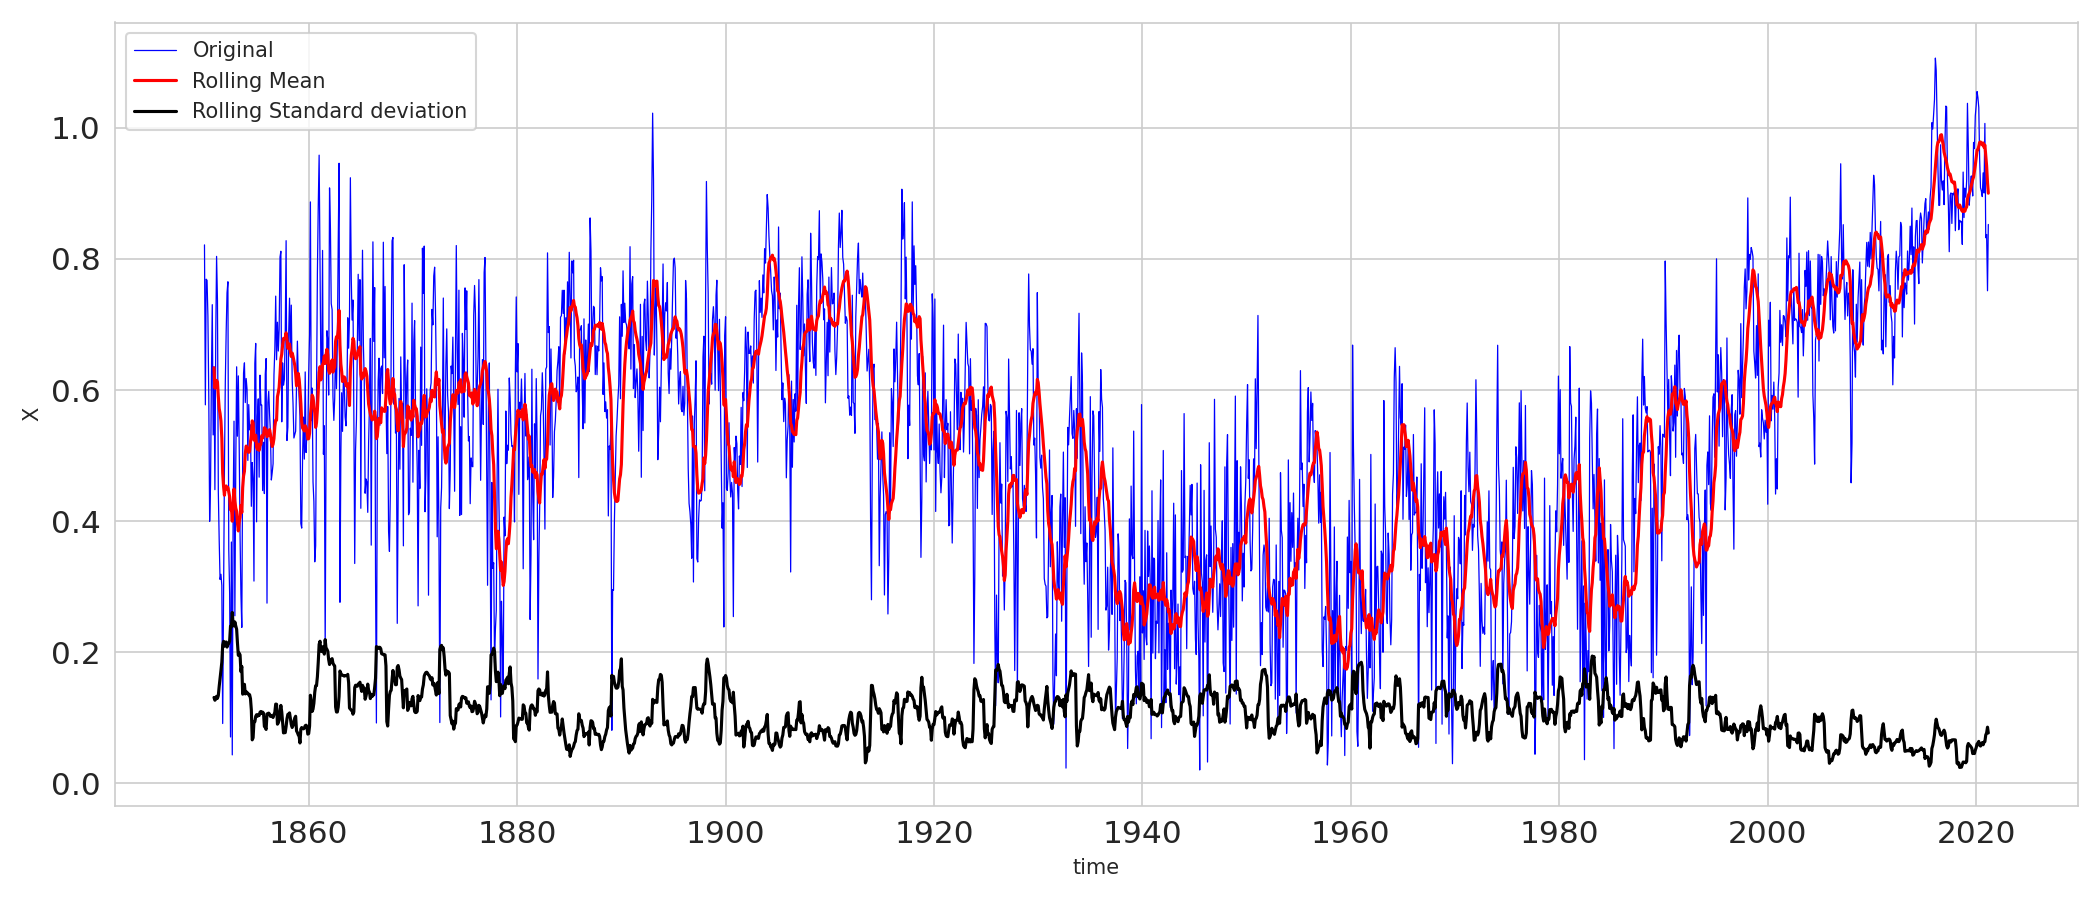
\includegraphics[width=1\textwidth]{images/ts_moving_avg_B.png}
			\caption{Average temperature anomaly raw data.}
			\label{fig:rollingmean_B}
		\end{figure}
		\begin{figure}
			\centering
			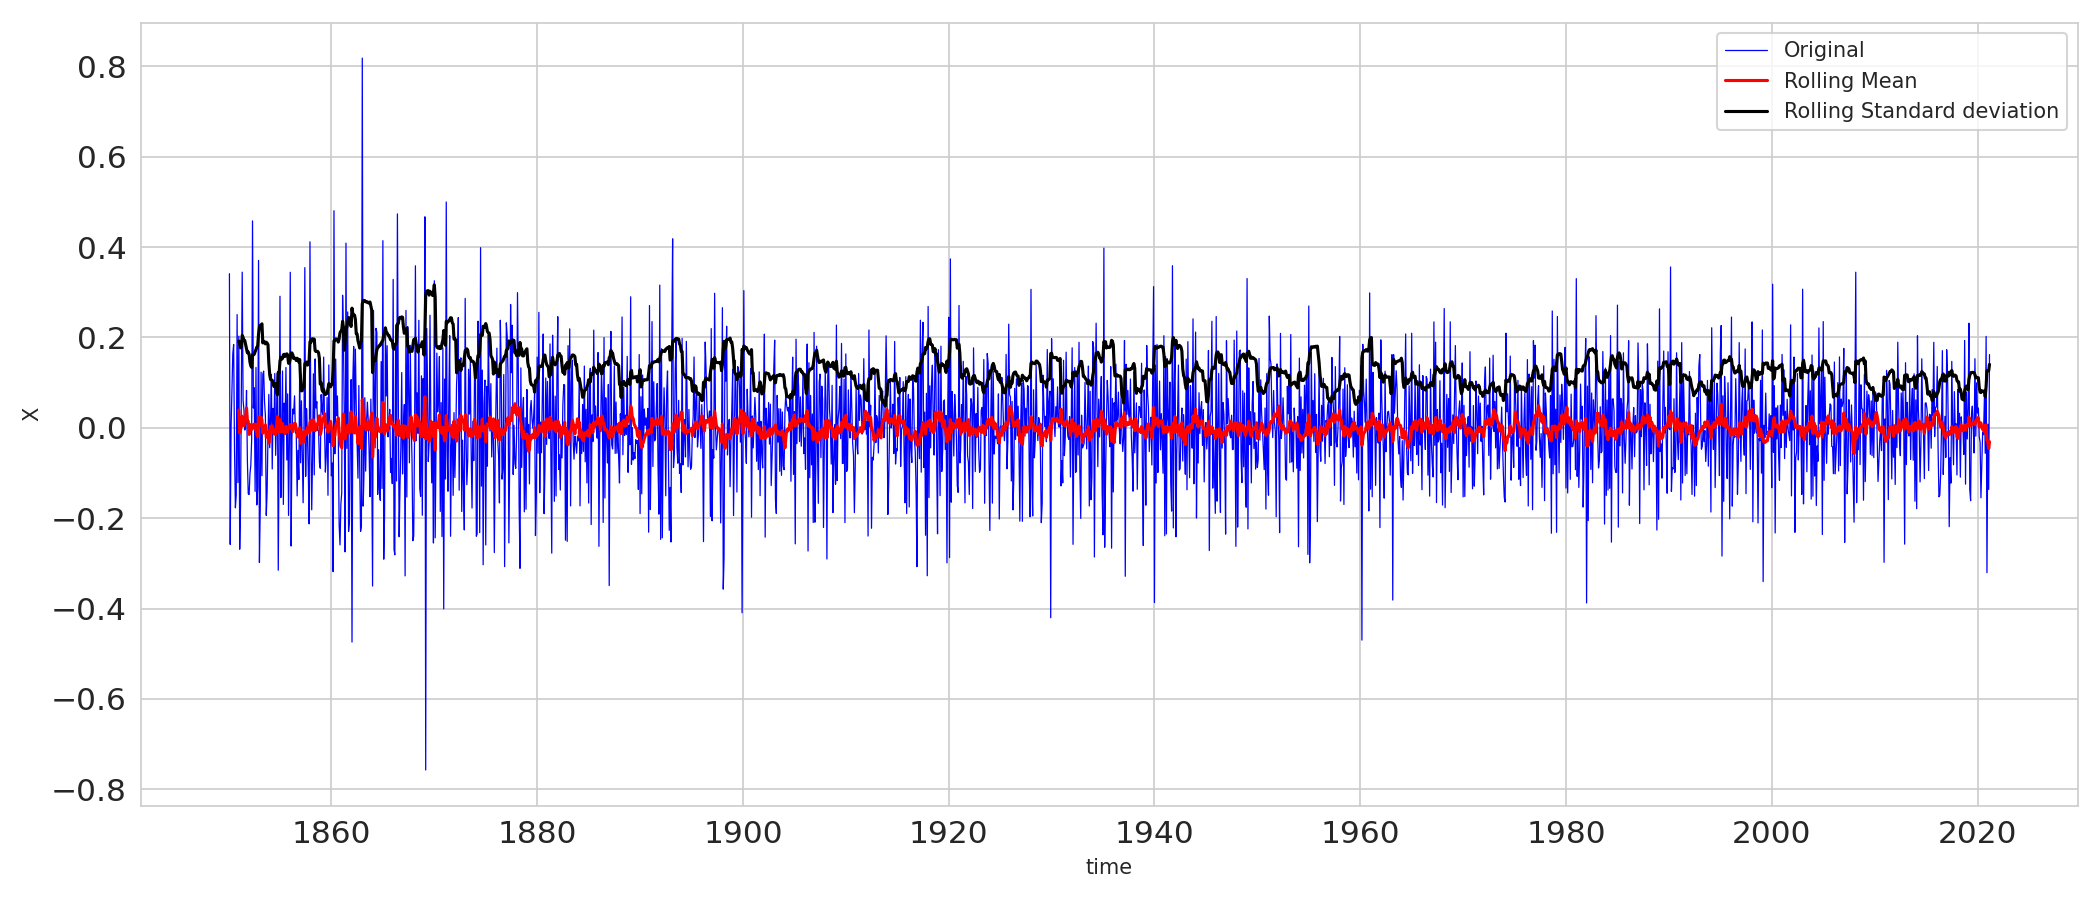
\includegraphics[width=1\textwidth]{images/ts_moving_avg_diff_B.png}
			\caption{Average temperature anomaly after differencing.}
			\label{fig:rollingmean_diff_B}
		\end{figure}
		\begin{figure}
			\centering
			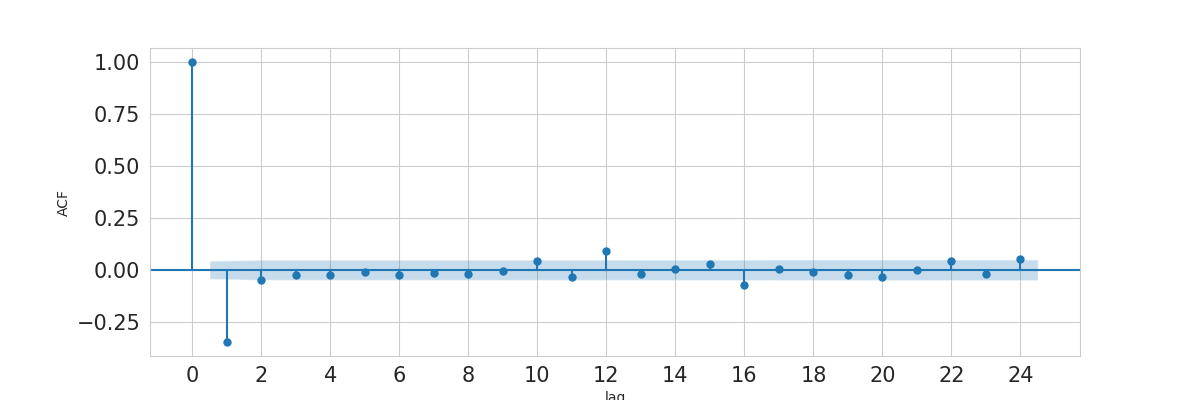
\includegraphics[width=1\textwidth]{images/autocorrelation_B.png}
			\caption{The autocorrelation function.}
			\label{fig:acf_B}
		\end{figure}
		\begin{figure}
			\centering
			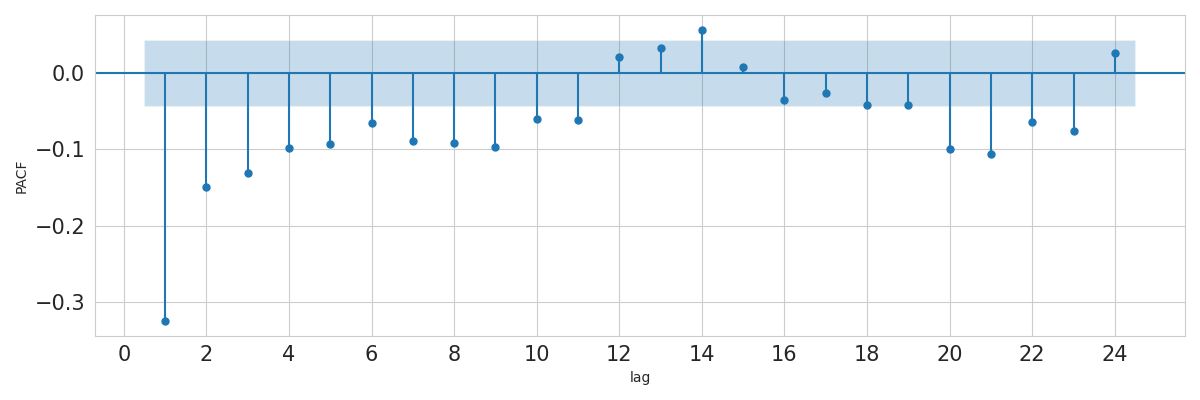
\includegraphics[width=1\textwidth]{images/partialautocorrelation_B.png}
			\caption{The partial autocorrelation function.}
			\label{fig:pacf_B}
		\end{figure}
		\begin{figure}
			\centering
			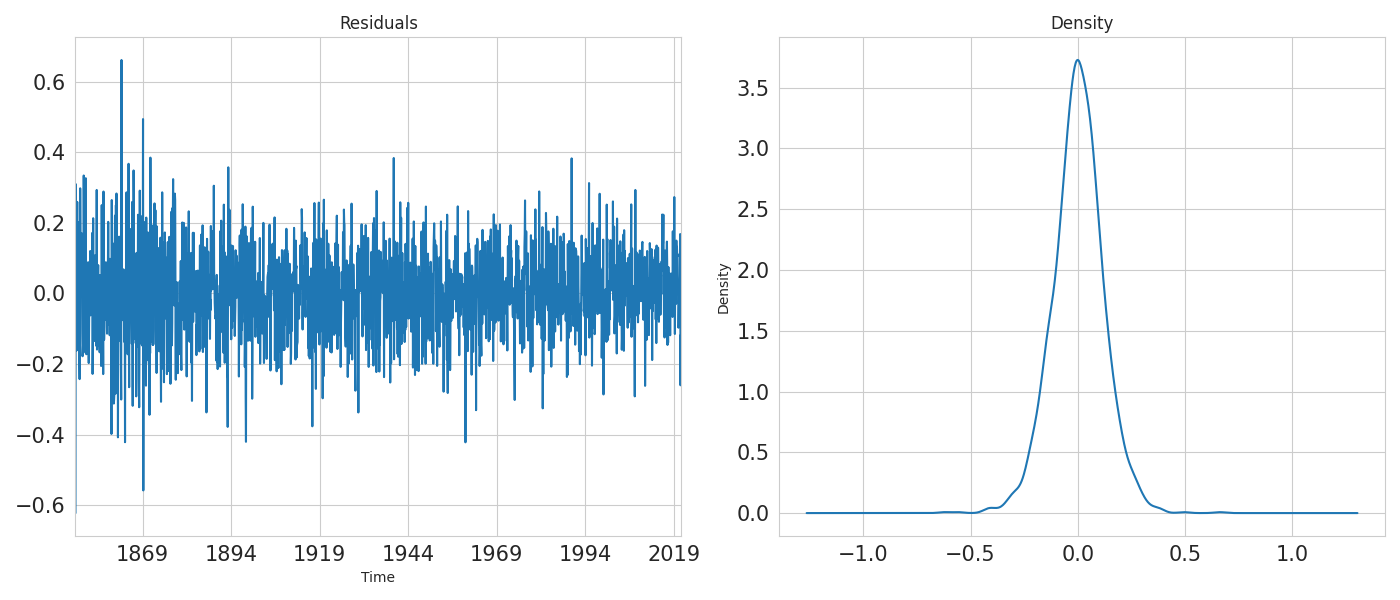
\includegraphics[width=1\textwidth]{images/res_dens.png}
			\caption{Residuals and density.}
			\label{fig:res_dens}
		\end{figure}
		\item
		\begin{figure}
			\centering
			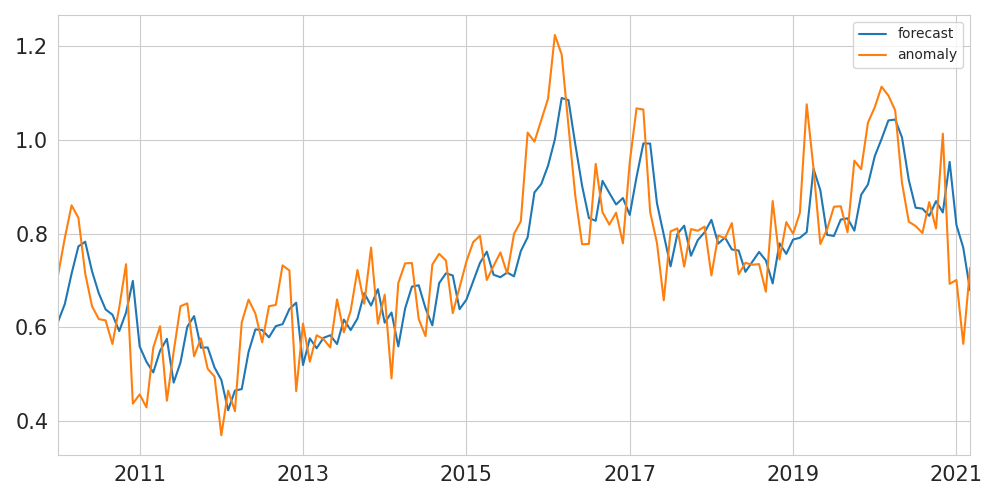
\includegraphics[width=1\textwidth]{images/forecast_2010-2021.png}
			\caption{Forecast 2010 - 2021}
			\label{fig:forecast_2010-2021}
		\end{figure}
		\begin{figure}
			\centering
			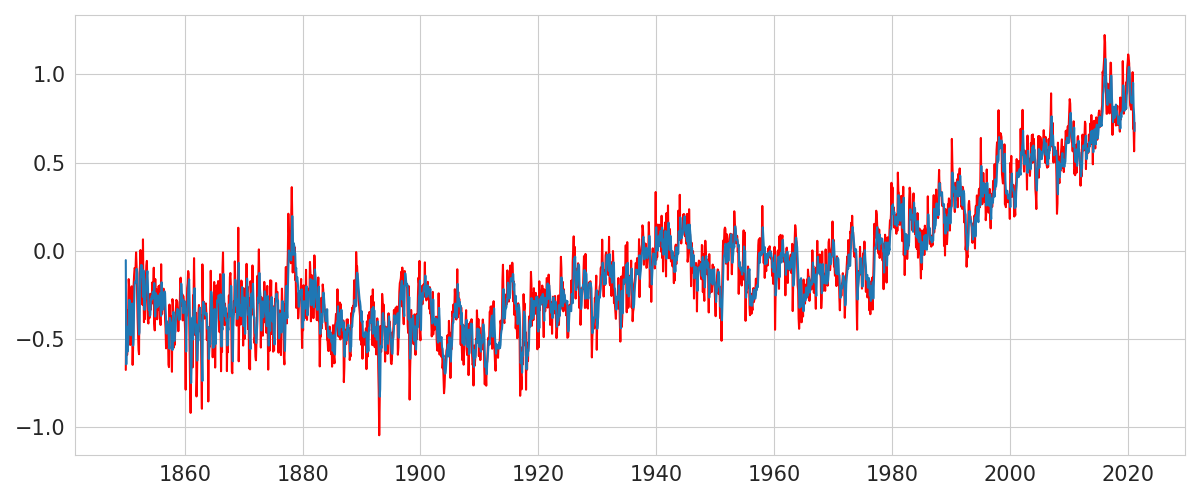
\includegraphics[width=1\textwidth]{images/forecast_2010-2021_RMSE.png}
			\caption{Forecast 2010 - 2021 RMSE}
			\label{fig:forecast_2010-2021_RMSE}
		\end{figure}
		\item
	\end{itemize}
	\section{Image classification}
	\subsection{Image classification}
	If better means higher accuracy then i would choose a CNN for image classification. RF performs well on categorical data while a CNN handles numerical input very well. Here we have pixels with numerical values between 0 and 255. We can also tune more parameters in a CNN like kind/number of layers, epochs and learning rate. Also different activation functions for the neurons can be chosen. Finally a CNN learns how to apply a filter to an input during training such that certain features in the image can be recognized. A RF can not take advantage of such structures in images.
	
	On the other hand a CNN needs a lot of data to perform well. I don't know exactly if our dataset is large enough but if i compare with other models they used hundred thousands or even millions of images to train a CNN.

	\subsection{Classification performance}
	\begin{itemize}
		\item Accuracy CNN: 99.00\%, that means the error rate was 1\%. It misclassified 10/1000 images from my test set.
		\item Accuracy RF: 90.5\%, that means the error rate was 0.5\%. It misclassified 5/1000 images from my test set.
		\item Both models performed surprisingly good. I checked many times if i excluded any test data from the training. No model performed significantly better.
		\item Both models agreed in all images only the CNN misclassified image 001212.jpg where it predicted the class 'headCT' instead of 'Hand'. As far as i can tell the RF made no prediction error on the unlabeled dataset.
		\begin{figure}
			\centering
			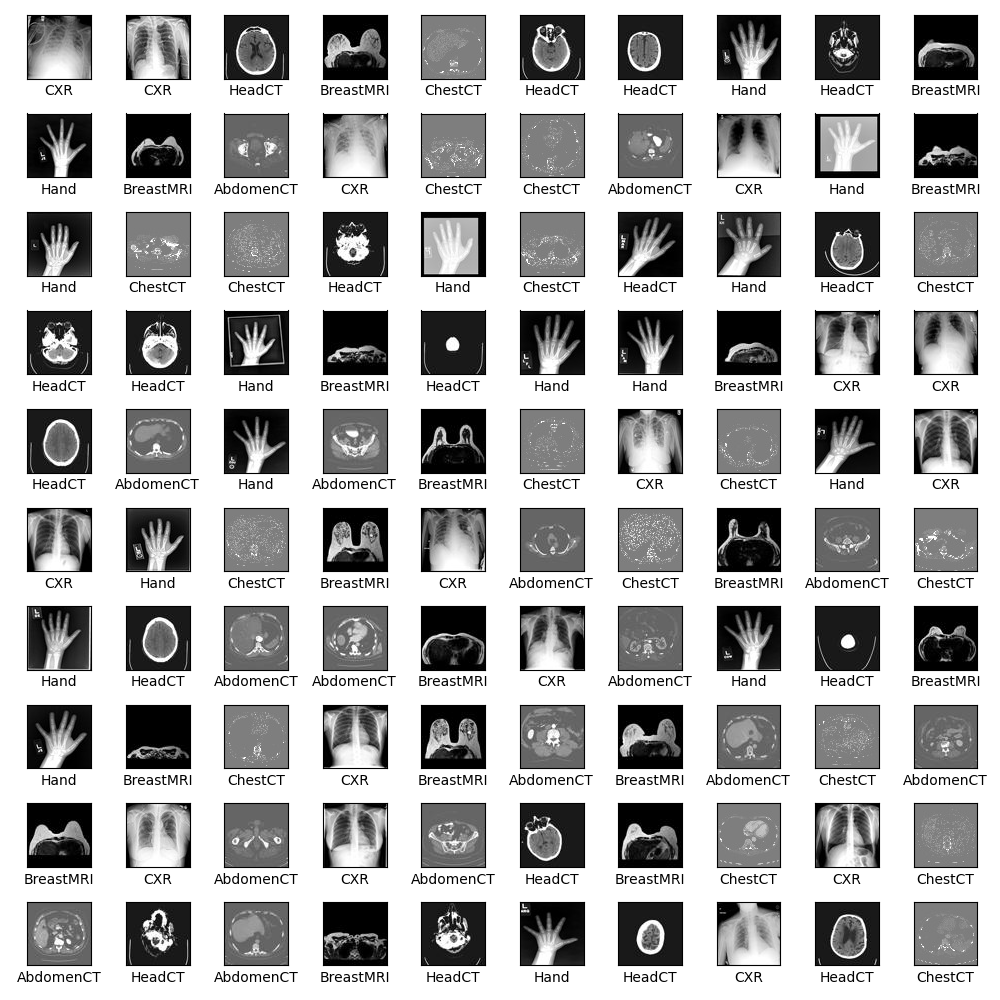
\includegraphics[width=0.8\textwidth]{images/pred_img_cnn.png}
			\caption{The prediction from the convolutional neural network. It misclassified one image. Can you find it?}
			\label{fig:pred_img}
		\end{figure}
		I included the corresponding files in the folder \texttt{report/data} in the repository (\texttt{predictions\_cnn.csv}, \texttt{predictions\_rf.csv}).
	\end{itemize}
	
	\subsection{Hyper parameter tuning}
	
	\subsection{Interpretation of model performance}
	\subsection{Bonus Question}
\end{document}